\documentclass[11pt]{article}
\usepackage[utf8]{inputenc}
\usepackage[toc,page]{appendix}
\usepackage{microtype}
\usepackage{fullpage}
\usepackage{multirow}
\usepackage{tocloft}

\usepackage[newfloat]{minted}
\usepackage{caption}
\setminted[]{linenos, numbersep=5pt, frame=lines}

\usepackage{parskip}
\setlength{\parindent}{0em}
\setlength{\parskip}{1em}

\newenvironment{code}{\captionsetup{type=listing}}{}
\SetupFloatingEnvironment{listing}{name=Source Code}

\usepackage{array}
\newcolumntype{L}{>{\centering\arraybackslash}m{1.2in}}
\newcolumntype{M}{>{\centering\arraybackslash}m{0.85in}}
\newcolumntype{N}{>{\centering\arraybackslash}m{0.5in}}
\usepackage{tablefootnote}

\usepackage[affil-it]{authblk}
\usepackage{amsfonts, amssymb, amsmath}

\usepackage{wrapfig}
\usepackage{graphicx}
\graphicspath{ {./images/} }

\usepackage{float}

\usepackage[backend=biber]{biblatex}
\addbibresource{sources.bib}
% Use the followign Command to validate *.bib file: biber --tool --validate-datamodel qualifying_exam_paper.bib

\title{Improving Emotion Detection through Translation of Text to ML Models Trained in Different Languages}

\author{Richard Hoehn%
	\thanks{Electronic address: \texttt{rhoehn@mtmail.mtsu.edu}; corresponding author}}
\affil{Middle Tennessee State University}

\author{Dr. Jaishree Ranganathan%
	\thanks{Electronic address: \texttt{jaishree.ranganathan@mtsu.edu}}}
\affil{Middle Tennessee State University}

\begin{document}

\maketitle

\begin{abstract}
This Qualifying Exam\footnote{Comp. and Data Science PhD students are required to complete a Qualifying Exam in their first year} research paper investigates enhancing Emotion Detection (ED) by translating extended text data into various Machine Learning (ML) models trained in distinct languages. We focused on English and German text data to enhance prediction accuracy, aiming to overcome challenges arising from limited labeled datasets and language fragmentation in ED research.

Expanding an original English dataset with translated German data increases the training data's volume, potentially improving prediction rates in ED applications. Additionally, translating English to German to extend the German dataset and accessing in real-time ML models trained in both could further improve prediction rates.

For presentation purposes, datasets in both English and German were collected, parsed, cleaned, and translated. Multiple ML models trained in English and German where built, and made accessible via an API for predictions in either language including real-time translation using a GET method.

The research findings suggest that the extension of datasets through translation has not yielded improvements in predictive accuracy for both English and German languages. Modest enhancements could potentially be achieved by concurrently accessing English and German models through real-time translation via the RESTful API; however, the benefits may not fully justify the efforts.

We posit that the prevalence of numerous classes in this multi-class classification model has contributed to instances of overfitting across several labels/classes. This occurrence, in turn, has led to a memorization effect rather than facilitating genuine learning within the models.

In conclusion, it becomes evident that a more substantial accumulation of data is required, or an innovative approach involving the utilization of AI to generate analogous data must be employed to comprehensively address this research question.
\end{abstract}
\clearpage

\tableofcontents

\clearpage
\section{Introduction}

Emotion detection (ED) has gained significant interest and investment\cite{Sarker2021} in recent years as a means to understand human behavior and improve communication effectiveness. By analyzing text, speech or facial expressions, these detection processes try to accurately identify and classify emotions expressed by individuals or groups, often in real-time.

By employing a variety of ED processes, including natural language processing (NLP) and machine learning (ML), applications with the right amount of data can detect emotions with high precision\cite{research-emotion-recognition-for-online-learning}. These ED systems find applications in diverse fields, such as sentiment analysis, customer feedback analysis, voting and news stance prediction, and mental health monitoring, which all aim at contributing to a deeper understanding of human emotions and their impact on various aspects of life.

\subsection{Human Emotion as a Theoretical Framework}
\label{sec:human-emotion-as-a-theoretical-framework}
The concept and number of emotions can vary depending on the theoretical framework or model being considered. One well-known model is the Plutchik's Wheel of Emotions seen in Figure \ref{fig:plutchik-wheel}, which proposes eight (8) primary emotions and their contrasting pairs. In this research paper we will be focusing on the basic eight (8) emotions and not on their sub-emotions or contrasting pairs. This allows the ML models being trained and built to be a multi-class classification model with eight labeled options.

The following are the eight primary emotions according to the Plutchik's Wheel of Emotions \cite{Tromp} that we will be focusing on both in our English and German datasets. A detailed reference of emotions used in this research can be found in Table \ref{table:dataset_labels} on page~\pageref{table:dataset_labels}.

\begin{itemize}
\item Happiness: A feeling of Joy (Fun), contentment, or delight.
\item Sadness: A state of unhappiness, sorrow, or grief.
\item Anger: An intense emotional response associated with feelings of displeasure, frustration, or hostility.
\item Worry: An emotional response triggered by perceived threats or danger, often associated with anxiety or terror.
\item Surprise: A sudden and unexpected reaction to something unusual or startling.
\item Disgust and/or Hate: A strong aversion or revulsion towards something unpleasant, offensive, or repulsive.
\item Trust and/or Love: A sense of reliance, confidence, or faith in someone or something.
\item Enthusiasm: A feeling of excited expectation or eagerness towards future events.
\end{itemize}

\begin{figure}[h]
    \centering
    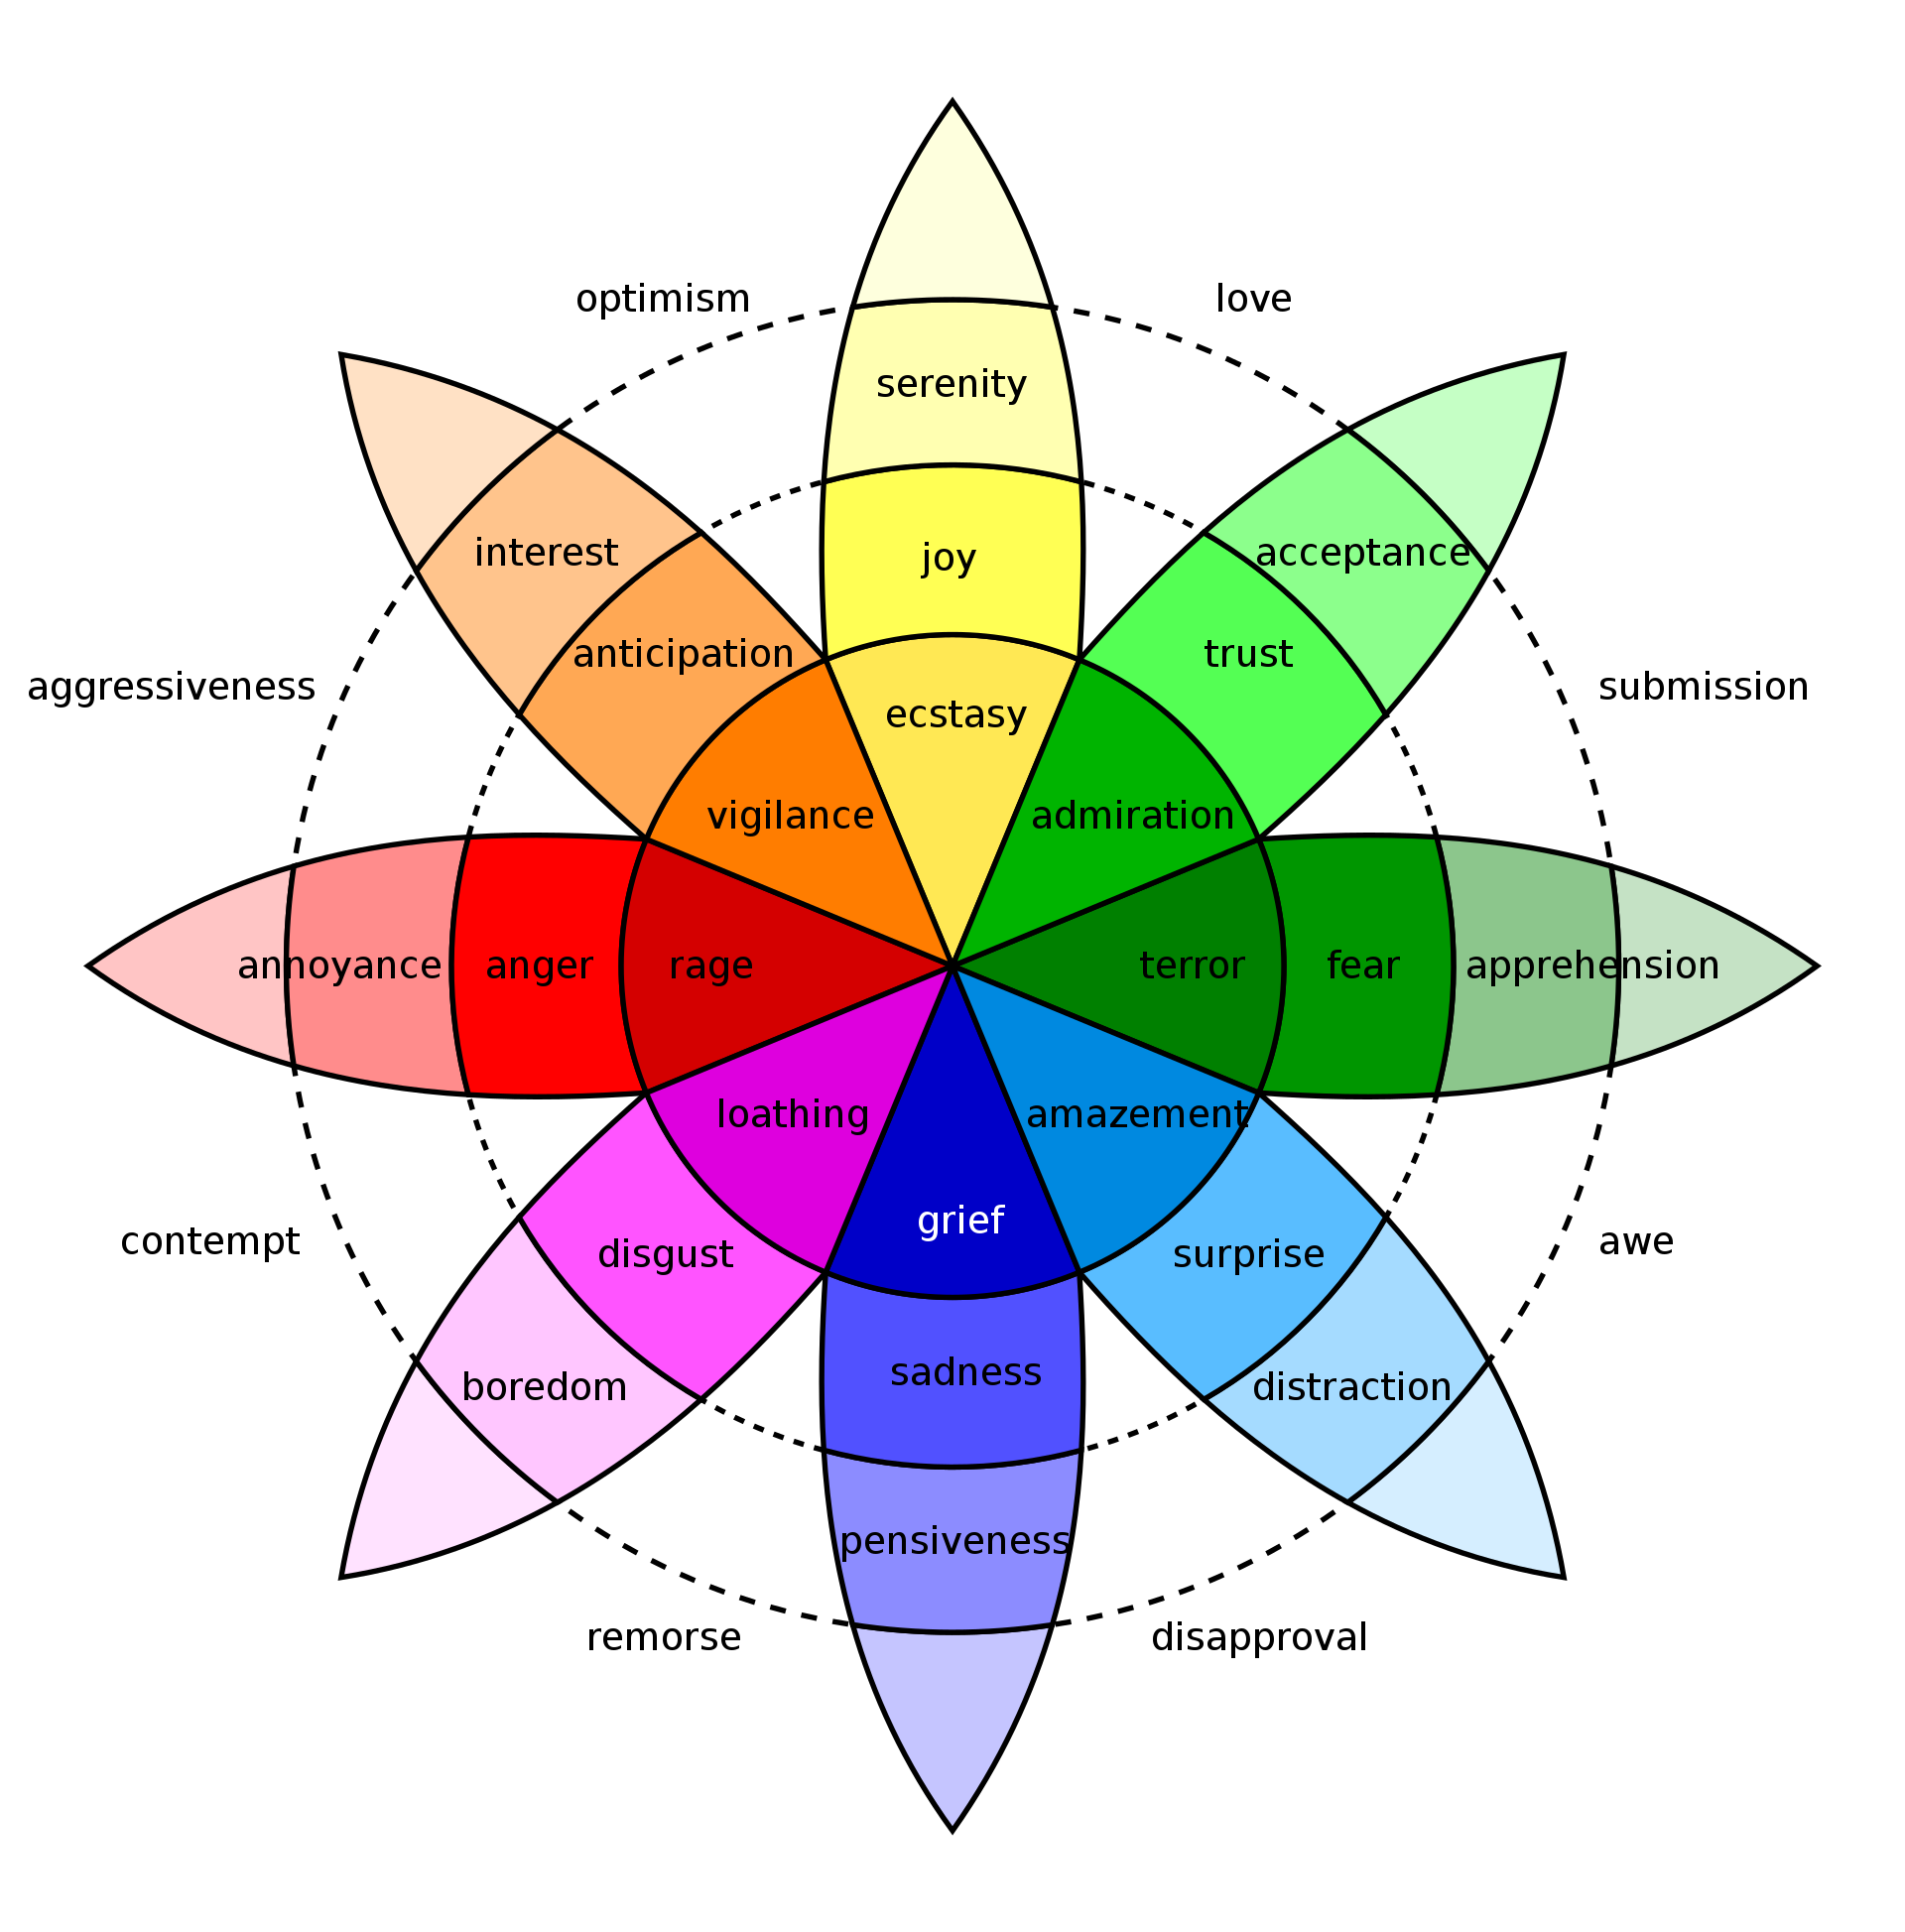
\includegraphics[width=0.4\textwidth]{Plutchik-Wheel}
    \caption{Plutchik Wheel of Emotions}
    \label{fig:plutchik-wheel}
\end{figure}

It's important to note that emotions are complex and multifaceted, and different emotion models and/or frameworks may propose alternative categorizations or variations in the number of primary emotions. However for the scope of this research project the most common eight (8) emotions are used as described above. This allows the ML models being trained and built to be a multi-class classification model with eight labeled classes.

By aligning the emotional labels across the English \cite{english-dataset-twitter} and German \cite{german-dataset-cheese} datasets that are being used in this research all eight listed above were linked to each other. Details on the linkage of the two datasets and their counts from data are described in Section \ref{sec:data-procurement-process} with an emphasis on Table \ref{table:dataset_labels}'s cross reference on page~\pageref{table:dataset_labels} of German and English language data.

\subsection{Significance of Emotion Detection in Machine Learning}
Emotion Detection (ED) analysis in Machine Learning (ML) models has gained significant attention due to its potential applications in various fields, including customer sentiment analysis, stance detection in regard to a specific targets such as news and voting\cite{mascarell-etal-2021-stance}, mental health monitoring\cite{Colonnello}, and human-computer interactions such as chat-bots\cite{chatbot-cognitive-awareness} to just name a few.

By accurately identifying and understanding emotions from text data, ML applications can assist in improving user experiences, decision-making processes, and overall human-machine interactions in a positive manner\cite{Colonnello, mascarell-etal-2021-stance}, with most of these interactions being processed in real-time.

As an example, the primary goals of chat-bots are entertainment, social contact, support, and novelty interaction, with a strong emphasis on productivity, scale-ability and cost reductions. In the case of chat-bots, there has been a immense requirement to simulate human-like characteristics and behaviors during human-machine interactions\cite{emotion-detection-literature-review}. Per Kusal et al. \cite{chatbot-cognitive-awareness} these chat-bots also improve customer engagement by offering friendliness, comforters, flexibility, and efficient assistance. As such chat-bots should provide customers with more engaging responses, directly addressing their issues or questions. The goal of deploying ED to these applications is for users perceive chat-bots as companions rather than simple assistants, which in turn helps the overall process of getting to a positive result. Per Adikari et al. the majority of user requests are emotional rather than informative; therefore the need for chat-bots to gain the capacity to respond emotionally to customers via machine learning and sentiment analysis evolution\cite{chatbot-cognitive-awareness} is very important and yields for many applications that use ED a way to improve interactions with machines.

\begin{quote}
    I usually know almost exactly how I feel. The problem is, I just can’t tell anyone.
    \flushright -- Meg Cabot
\end{quote}

Due to the above mentioned wide scope of uses for ED this field of research and the work to advance it provides significance and importance in enabling machines to comprehend and respond appropriately to human interactions. Our research in turn contributes to the advancement of artificial intelligence, natural language processing (NLP) and in many cases the utilization of text-to-speech applications most all of us in today's society use and rely on \cite{ai-framework-detection-emotions} to go about our daily lives.

Lastly, in the paper by Chen et al.\cite{research-emotion-recognition-for-online-learning} based on emotion detection for online learning it states, interestingly, that with emotion recognition research, we need to focus on accuracy and real-time performance in order to apply ED based on physiological signals to solve practical problems; the key part of their claim is that in order for ED to be practical, real-time methods need to be used and deployed for maximum results.

\subsection{Challenges: Lack of Labeled Datasets and Language Fragmentation}
Emotion Detection is a fast growing field\cite{ACLU-ED-Data, ACLU-THE-DAWN-OF-ROBOT-SURVEILLANCE}, however unlike Sentiment Analysis (SA) the availability of large datasets for training purposes of ML models is much smaller \cite{ACLU-ED-Data, ai-framework-detection-emotions}. The primary reason of the lack of data stems from the face that emotion detection data requires primarily supervised learning data. In turn requires time and effort to construct, catalog, and procure,; this all is mostly created and labeled by humans. To compound on the issue of the lack of labeled data; the many datasets that are available are in many cases in multiple languages - not all are in English since emotions that are linked to text are contextual in nature. for this research a a significant amount of time took place to find the German labeled data, which eventually was found online by google searching.

\subsection{Motivation for the research project focusing on extending ED datasets through translation and evaluating the impact on prediction rates}

This paper is significant because an entire industry of automated emotion reading (Text, Image, Video, and Sound) technologies is quickly emerging \cite{ACLU-ED-Data, ACLU-THE-DAWN-OF-ROBOT-SURVEILLANCE}. The market for emotion recognition and detection software is forecast to reach at least \$3.8 billion by 2025 \cite{ACLU-ED-Data, ACLU-THE-DAWN-OF-ROBOT-SURVEILLANCE}. And since ED is already being incorporated into products for purposes such as marketing, robotics, driver safety, customer service, news and stance analysis, and a multiple of others, it is fitting to work on research to solve and / or improve issues in regards to prediction rates due to lack of data and language fragmentation.

With the above mentioned issues regarding the quantity (lack of) and language fragmentation of the ED datasets this research was motivated by finding a way to combine different language datasets into a single set for training processes to improve the predictability of ED. The aim of the research is that by use of translation that the predictability of ED can be improved by extending an English dataset with translations from German and also process look-ups in real-time language conversion and processing.

\subsection{Objectives \& Scope of the Research}

The primary objective of this Qualifying Exam research project is to address three (3) research questions, each aimed at improving the accuracy of predictive ED models in the context of English and German language datasets.

\begin{itemize}
\item The first hypothesis is that by introducing English data translated into German and extending an original German dataset, will the added text lead to an enhancement in its predictive capabilities. (Section \ref{sec:analysis-of-impact-of-extending-datasets})
\item Similar to the first, can by translating German data to English and extending an original English dataset increase the predictability of English ED model? (Section \ref{sec:analysis-of-impact-of-extending-datasets})
\item The third research question shifts the focus to real-time translation and its impact on prediction. Can by translating in real-time an input to multiple languages improve the predictability based on the combined output of two models that were trained in English and German to better the prediction results. (Section \ref{sec:impact-using-api-for-real-time-translation})
\end{itemize}

In summary, this research project centers around investigating innovative ways to enhance the predictability of Emotion Detection models in both English and German. With these three (3) objectives from above our methodology will be to procure, translate, train, and evaluate benefits of extending datasets by translation to improve emotion detection. 

\clearpage
\section{Literature Review}
To ensure comprehensive coverage of the latest developments and research in emotion detection and analysis for this research paper, consideration and review was only given to incorporating research papers and online news articles that were published after the year 2015, thereby providing an up-to-date perspective on the subject matter at hand.

We believe by implementing the 2015 boundary, our methodology and results aim to provide a more up-to-date outlook on the subject matter at hand and what areas the emotion detection field is moving in with respect to machine learning research, applications and processes.

\subsection{Emotion Detection Importance and Diverse Populations}
Emotion Detection (ED) holds significant importance\cite{Sarker2021} in various domains, including psychology, social sciences, and human-computer interaction. By use of ML models\cite{CHOWANDA-2021821} the analysis of human emotions at scale, providing valuable insights into individual and collective emotional states both in real-time but also as a type barometer for measuring sentiments from the past versus the current time. In Chowanda et al. paper\cite{CHOWANDA-2021821} they believe that "Emotions hold a paramount role in the conversation, as it expresses context to the conversation.", this means that emotions are a part of a conversation and with that are needed to ensure valid analysis of a conversation.

Furthermore Kapoor et al. \cite{KAPOOR2023120882} states that, emotions can differ across age groups, genders, cultures, and languages. Including data from diverse populations helps in developing inclusive and culturally sensitive ED models. It ensures that the models are not biased towards specific groups and can accurately detect emotions in a wide range of individuals.

\subsection{Lack of Labeled Datasets and Fragmentation caused by Different Languages}
The lack of diverse and large-scale data hinders the development and training of accurate ED models, limiting their effectiveness and general ability across different contexts and populations. In recent research, efforts have been made to address these limitations by exploring new techniques for emotion detection.

For instance, a study by Kapoor\cite{KAPOOR2023120882} et al. proposes analyzing the entire spectrum of the language source to predict emotional changes. This provided some help, but quickly established itself as time consuming task and need of expertise in the subject matters that could not outweigh the results. Overcoming the scarcity of labeled datasets and embracing innovative approaches like the above mentioned study by Kapoor\cite{KAPOOR2023120882} et al. and their analysis can contribute to the advancement of ED research. Such advancements hold the potential to enhance the accuracy and applicability of emotion detection models, enabling a deeper understanding of human emotions and more effective responses in various domains, although the cost of such might be prohibitive at this time.

In addition, the paper by Mascarell\cite{mascarell-etal-2021-stance} et al. states that unlike images language operate very differently, therefore the lack of labeled datasets poses a significant challenge in text-based Emotion Detection (ED) analysis as it limits the availability of reliable training data for ML models. This scarcity hampers the model's ability to learn and generalize emotions effectively.

And lastly, a paper by Kusal et al. further stipulates \cite{kusal} that the fragmentation caused by different languages further exacerbates the issue, as it reduces the size and diversity of data available for training, resulting in limited cross-lingual generalization and potentially biased models.

Overcoming these challenges, lack of data and language fragmentation, is crucial for advancing emotion detection and analysis research for improving the accuracy, speed, and applicability of ML models across various languages and cultures.

\clearpage
\section{Methodology}

\subsection{Data Procurement and Parsing of ED datasets in English and German}
\label{sec:data-procurement-process}
The data procurement was relatively straight forward and once found by using multiple Google search terms for the Emotion Detection in English and German text languages. Some of the main German data was obtained from the dataset built by ETH's Emotion and Stance Detection for German Text \cite{mascarell-etal-2021-stance} which also hosts a good website with their findings\footnote{https://mtc.ethz.ch/research/natural-language-processing/emotion-stance.html}. The English dataset was downloaded from Kaggle\footnote{https://www.kaggle.com/datasets/pashupatigupta/emotion-detection-from-text} based on Tweets collected in 2021. The English dataset contains over 38,000 tweets and their corresponding emotion's labeled. Unfortunately the German dataset only contained just over 2,500 sentences and their respective emotions associated with it. Unfortunately this imbalance (see Table \ref{table:file-details}) of the two dataset sizes will had to be corrected and is explained in detail in the subsequent sections.

\begin{table}[h!]
\centering
\begin{tabular}{ | c | c | c | }
    \hline
    \multicolumn{3}{|c|}{File Details} \\
    \hline
    Name & Row Count & Type \\
    \hline
    English & 38,000 & CSV  \\
    German  &  2,500 & JSON \\
    \hline
\end{tabular}
\caption{File details of English \& German data.}
\label{table:file-details}
\end{table}

An important part of the process is to make sure we match / link the English emotions to those of the German language emotions. Since the two languages are dissimilar we opted to match exact emotions to each other that can be seen in Table \ref{table:dataset_labels} below. The linking yielded our eight (8) emotions we previously discussed in Sections \ref{sec:human-emotion-as-a-theoretical-framework}. Details on how we formatted the the two (English and German) datasets to each other can be viewed in the Appendix \ref{appendix:dataset_english} and \ref{appendix:dataset_german}.

\begin{table}[h!]
\centering
\begin{tabular}{ | c c | c c | c | }
    \hline
    \multicolumn{5}{|c|}{Emotion Datasets Labels} \\
    
    \hline
    \multicolumn{2}{|c|}{English} & \multicolumn{2}{c|}{German} & \multirow{2}{*}{Used} \\
    Name & Count & Name & Count \\
    \hline
    Boredom    &  179 & ---           & --- & NO  \\
    Love       & 3842 & Vertrauen     & 316 & YES \\
    Relief     & 1526 & ---           & --- & NO  \\ 
    Fun        & 1776 & ---           & --- & NO  \\
    Hate       & 1323 & Ekel          &  29 & YES \\
    Neutral    & 8638 & Unklar        & 314 & YES \\
    Anger      &  110 & Ärger         & 226 & YES \\
    Happiness  & 5209 & Freude        & 140 & YES \\
    Surprise   & 2187 & Überraschung  & 369 & YES \\
    Sadness    & 5165 & Traurigkeit   & 184 & YES \\
    Worry      & 8459 & Angst         & 154 & YES \\
    Enthusiasm &  759 & Antizipation  & 774 & YES \\
    Empty      &  827 & ---           & --- & NO  \\
    \hline
\end{tabular}
\caption{Dataset of English \& German and their respective label counts.}
\label{table:dataset_labels}
\end{table}

The processing of two ED datasets to be synchronized or linked to the emotion is important. The first will be in English and the second in German. Each dataset will be translated into the other's language for extension purposes. 

We decided to build the data to support that each row of each dataset will hold the English and German sentence. As an example Figure \ref{fig:dataset-extension} depicts the original English dataset will be extended by the translated German (German $\Rightarrow$ English) dataset. By this simple process the English dataset got larger for training purposes.

\begin{figure}[h]
    \centering
    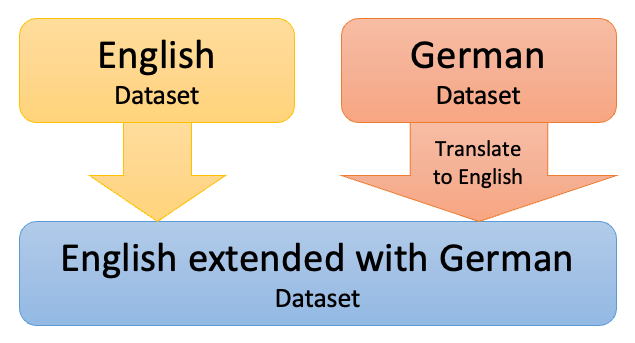
\includegraphics[width=0.4\textwidth]{Dataset-Extension}
    \caption{Example of English dataset extension by translating from German.}
    \label{fig:dataset-extension}
\end{figure}

The reason for selecting German in this research project was based on the author\footnote{Richard Hoehn} being fluent in English and German and hence being able to easily traverse the two languages while working on the code for dataset translations and formatting. It was much easier to create the emotion cross reference Table \ref{table:dataset_labels} and also check the translation results due to the dual language benefit.

Once the two datasets have been translated, we now extend the original language dataset with the translated one. By this approach we are in essence extending the original datasets to create a larger one with the foreign language data. With both extended datasets we can now train our ML models for English and German.

\subsection{Translation Application for Converting English to German and Vice Versa}
Translation of the emotion datasets was performed with Google Translator based on the Medium article\cite{Nidhaloff_how_to_translate_text_with_python} in which the author describes options for simple API translations. Google Cloud Translation was use mainly due to it's free nature and ease of use for this project. There are however many other text based API translation services that could have been used and might yield in some circumstance even better results.

As an example the following is a brief introduction to Google Translator's API with the code snippet below depicting the ease of use to translate text via an API.

\begin{code}
\centering
\begin{quote}
\begin{minted}[samepage, fontsize=\small]{python}
# Using Deep Translator to leverage Google Translate
# Link: https://cloud.google.com/translate/docs/reference/libraries/v2/python
from deep_translator import GoogleTranslator

sentence = 'Chocolate milk is so much better through a straw.'

translated = GoogleTranslator(source='auto', target='de').translate(sentence)
print(translated) # Schokoladenmilch schmeckt durch einen Strohhalm viel besser.

translated_back = GoogleTranslator(source='auto', target='en').translate(translated)
print(translated_back) # Chocolate milk tastes much better through a straw.
\end{minted}
\captionof{listing}{Google Translate Example Code}
\end{quote}
\end{code}

Based on the above translation example the CSV\footnote{CSV = Comma Separated Values} (English) and JSON\footnote{JSON = JavaScript Object Notation} (German) datasets were individually loaded, parsed, and translated to their respective counter-part languages. Details of the application can be found in the Appendix \ref{appendix:dataset_english} for English and Appendix \ref{appendix:dataset_german} for the German processing. We decided to only use 1,500 rows from each language. This decision was made since the German (DE\footnote{DE = German}) dataset was not much larger than that once filtering and processing was completed. This meant that the English (EN\footnote{EN = English}) dataset was randomly paired down to 1,500 to match that of the German. 

Each translated file now contains four (4) columns that are labeled in Tables \ref{table:pd_de_translated} and \ref{table:pd_en_translated} with the exact same column naming.

\begin{table}[h!]
\centering
\begin{tabular}{ | L | L | L | L | }
    \hline
    \multicolumn{4}{|c|}{File: \texttt{pd\textunderscore de\textunderscore translated.csv}} \\
    \hline
    sentence\textunderscore de &
    emotion\textunderscore de & 
    sentence\textunderscore en & 
    emotion\textunderscore en \\
    \hline
    Original Sentence (feature) &
    Original Emotion (label) &
    Sentence Translated to English & 
    Emotion set by Cross-Reference from German \\

    \hline
\end{tabular}
\caption{German CSV file structure after translation to English}
\label{table:pd_de_translated}
\end{table}

\begin{table}[h!]
\centering
\begin{tabular}{ | L | L | L | L | }
    \hline
    \multicolumn{4}{|c|}{File: \texttt{pd\textunderscore en\textunderscore translated.csv}} \\
    \hline
    sentence\textunderscore en &
    emotion\textunderscore en & 
    sentence\textunderscore de & 
    emotion\textunderscore de \\
    \hline
    Original Sentence (feature) &
    Original Emotion (label) &
    Sentence Translated to German & 
    Emotion set by Cross-Reference from English \\

    \hline
\end{tabular}
\caption{English CSV File structure after translation to German}
\label{table:pd_en_translated}
\end{table}

\subsection{Training Multiple ML models with PySpark}
After the completion of translating and processing the English and German datasets we come to training our models. Using the datasets from Tables \ref{table:pd_de_translated}, \ref{table:pd_en_translated}, and \ref{table:ml_models} that list an approximate $\sim$1,275 and $\sim$2,775 features for training.

It is important to note that in order to accurately test and compare the original and the extended datasets to each other we made sure that the test data was the same on each case. To do this we randomly extracted 15\% of the original datasets (English and German) and saved it as a test dataset prior to extending the original with the translated sentence data.

\begin{code}
\centering
\begin{quote}
\begin{minted}[samepage, fontsize=\small]{python}
# Split the English and German Dataframes for Training and Testing
# We are using a 15/85 Split
df_en_train, df_en_test = df_en.randomSplit([0.85, 0.15], seed=2023)
df_de_train, df_de_test = df_de.randomSplit([0.85, 0.15], seed=2023)

# Create the Extended Dataframe with Translated Data
# It is important to add the translated to the training data and not all of it
# Using *df_en_train.columns ensure that the columns are matched with the union
df_en_train_extended = df_en_train.union(df_de.select(*df_en_train.columns))
df_de_train_extended = df_de_train.union(df_en.select(*df_de_train.columns))
\end{minted}
\end{quote}
\captionof{listing}{Linking the English and German Emotions to the same label}
\end{code}

In Chowanda et al. paper\cite{CHOWANDA-2021821} on Text-based Emotion Techniques multiple algorithms were proposed, our research focused on just three (3) out of the six from the paper since the others had lower prediction rates based on the paper\'s conclusions. The algorithms tested in this research project ranged from the traditional machine learning to deep learning techniques, they are:
 \begin{itemize}

\item \textbf{Na\"ive Bayes:} Per Pujan's paper\cite{naive-bayes-model} on the Na\"ive Bayes model, it classifies and/or assigns the most likely class to a given example based on its feature vector, simplifying the task greatly by assuming that the features are independent given a class. 

\item \textbf{Generalised Linear Model (GLM):} Per Mueller's paper on GLM\cite{glm-model} the Generalized linear models extend the concept of the well understood linear regression model.

\item \textbf{Random Forest Classifier:} Per Schonlau's paper\cite{random-forest-model} on the Random Forest Classifier, they state that random decision forests easily adapt to non-linearity found in the data and therefore tend to predict better than linear regression. More specifically, ensemble learning algorithms like random forests are well suited for medium to large datasets.

\end{itemize}
 
Each of these algorithms used and their results are listed in the Results and Analysis Section \ref{sec:results-and-analysis} below.

 \begin{table}[h!]
\centering
\begin{tabular}{ | L | L | L | L | }
    \hline
    \multicolumn{4}{|c|}{ML Models } \\
    \hline
    Model & 
    Data &
    Rows for Training (85\%) & 
    Rows for Testing (15\%)  \\
    \hline
    A &
    English Original &
    1,275 & 
    225 \\
    \hline
    B &
    English Extended By German &
    2,775 & 
    225 same as Model "A" \\
    \hline
    C &
    German Original &
    1,275 & 
    225 \\
    \hline
    D &
    German Extended By English &
    2,775 & 
    225 same as Model "C" \\
    \hline
\end{tabular}
\caption{ML Models and their respective Train and Test Rows}
\label{table:ml_models}
\end{table}

The results of the testing resulted in some interesting parts that can be viewed in Table \ref{table:ml-prediction-result-versus-test-data}. We grouped the label by count from the test data (both English and German) and compared the predicted result counts to those. It became very clear that there was a strong bias on the GLM (Linear Regression) model that essentially proposed that all sentences evaluated to the same output both in English and German. 

\subsection{Creating an API for Translation and Parallel Processing}
\label{sec:create-api-for-translation-and-parallel-processing}

In order for a user to access and get prediction results from all three (Random Forest, Naives Bayes, and Linear Regression) ML models trained in both English and German in real-time we crated a Jupyter Notebook that starts an Apache PySpark\footnote{PySpark: https://spark.apache.org/docs/latest/api/python/index.html} session that is accessed via the local server listen on \texttt{https://127.0.0.1:8080}. The details of the RESTful the server can be found in Appendix \ref{appendix:code-api-server}.

The server listens for GET requests and evaluates a querystring either called \texttt{sentence\_en} or \texttt{sentence\_de} if an English sentence is sent then the server translates to German and if a German is sent then it translates to English. Each sentence is then tokenized, formatted, and processed on the previously trained ML models in both languages.

Once all the the ML model predictions have completed, we then lookup the emotion associated with the individually predicted labels and build a response \texttt{JSON} object to pass back the calling application. The \texttt{JSON} object (Source Code: \ref{code:json-object}) contains the original sentence and translated, plus each emotions predicted label by the six previously trained models. In addition the main data, and \texttt{metadata} object is created that holds the PySpark version, start, and end times, including the processing time in seconds.

\begin{code}
\begin{quote}
\begin{minted}[samepage, fontsize=\small]{json}
{
  "metadata": {
    "datetime": {
      "elapsed": 1.651038,
      "end": "Mon, 14 Aug 2023 12:10:35 GMT",
      "start": "Mon, 14 Aug 2023 12:10:33 GMT"
    },
    "spark": "3.3.2"
  },
  "predictions": {
    "de_lr": "enthusiasm",
    "de_nb": "relief",
    "de_rfc": "enthusiasm",
    "en_lr": "neutral",
    "en_nb": "love",
    "en_rfc": "happiness"
  },
  "sentence": {
    "english": "What a wonderful world this is!",
    "german": "Was für eine wundervolle Welt das ist!"
  }
}
\end{minted}
\captionof{listing}{JSON output from API}
\label{code:json-object}
\end{quote}
\end{code}

\subsection{Evaluation Metrics and Methodologies for Measuring the Performance}
\label{sec:evaluation-metrics-and-methodologies}
The evaluation of ML models trained on the English, German and their respective extension datasets is a critical step in assessing their performance and reliability. We chose to use the MulticlassClassificationEvaluator\footnote{URL: https://spark.apache.org/docs/latest/api/python/reference/api/pyspark.ml.evaluation.MulticlassClassificationEvaluator.html} because is a well known tool in the field of natural language processing (NLP) research, specifically in multi-class classification tasks such as emotion detection that has multiple labels associated with it; in our case eight (8) see Table \ref{table:dataset_labels} on Page \pageref{table:dataset_labels}. Generally this evaluator is used to evaluate the performance of machine learning (ML) models, using transformer-based architectures like BERT, RoBERTa, or DistilBERT\cite{Sanh2019-DistilBERT-AD}, with DistilBERT\cite{Sanh2019-DistilBERT-AD} being the one we used in this research project.

\begin{table}[h!]
\centering
\begin{tabular}{ | M | M | M | M | M | M | }
    \hline
    \multicolumn{6}{|c|}{ML Models Test versus Test Result Counts} \\
    \multicolumn{6}{|c|}{} \\
    \multicolumn{6}{|c|}{English} \\
    \hline
    ID & 
    Label &
    Test Data &
    NB Res & 
    GLM Res  &
    RFC Res \\
    \hline
    0 & boredom     &  0 & 25 \tablefootnote{In the NB a result that cannot be matched is a zero label} &   0 &   0 \\
    1 & love        & 26 &  8 &   3 &  11 \\
    2 & Relief      &  0 & 33 &   0 &   0 \\
    3 & Fun         &  0 &  5 &   0 &   0 \\
    4 & hate        &  9 & 31 &   0 &   0 \\
    5 & neutral     & 50 & 21 & 152 & 101 \\ 
    6 & anger       &  0 & 36 &   0 &   0 \\
    7 & happiness   & 39 & 44 &   5 &  17 \\
    8 & surprise    & 10 &  9 &   0 &   1 \\
    9 & sadness     & 29 &  0 &   2 &  19 \\
    10 & worry      & 46 &  0 &  50 &  63 \\
    11 & enthusiasm &  3 &  0 &   0 &   0 \\
    \hline
    \multicolumn{6}{|c|}{} \\
    \multicolumn{6}{|c|}{German} \\
    \hline
    ID & 
    Label &
    Test Data &
    NB Res & 
    GLM Res  &
    RFC Res \\
    \hline
    0 & boredom     &  0 & 34 &   0 &   0 \\
    1 & love        & 25 &  5 &   0 &  13 \\
    2 & Relief      &  0 & 28 &   0 &   0 \\
    3 & Fun         &  0 & 16 &   0 &   0 \\
    4 & hate        &  5 & 16 &   0 &   2 \\
    5 & neutral     & 30 & 24 &   0 &   5 \\ 
    6 & anger       & 23 & 20 &   1 &   7 \\
    7 & happiness   & 10 & 20 &   0 &   5 \\
    8 & surprise    & 24 & 47 &   0 &  11 \\
    9 & sadness     & 12 &  0 &   0 &   2 \\
    10 & worry      &  9 &  0 & 209 &   4 \\
    11 & enthusiasm & 72 &  0 &   0 & 161 \\
    \hline
\end{tabular}
\caption{Prediction Results Count compared to Test Data Label Counts}
\label{table:ml-prediction-result-versus-test-data}
\end{table}

The MulticlassClassificationEvaluator provides the essential evaluation metrics, including accuracy, Precision (eq: \ref{eq:precision}), Recall (eq: \ref{eq:recall}), and F1 Score (eq: \ref{eq:f1-score}) for ED classifications. These metrics provide valuable insights into a model's ability to correctly classify emotions across multiple classes and languages. Our research project is no different and the following measurements were used for our analysis:
\begin{itemize}

\item \textbf{Accuracy:} Accuracy measures the overall correctness of the emotion predictions made by the model. It is calculated as the ratio of correctly classified instances to the total number of instances in the dataset.

\item \textbf{F1 Score:} Precision represents the proportion of correctly predicted emotions among all instances predicted as a specific emotion with respect to the labels. Recall measures the proportion of correctly predicted emotions among all instances that truly belong to a specific emotion. With these two the F1 Score ($F1_{Score}=\frac{\text{Precision} \times \text{Recall}}{\text{Precision} + \text{Recall}}$) combines precision and recall into a single metric, providing a balanced evaluation.

\end{itemize}

While evaluating the models we focused on the Accuracy and the F1 Score to illustrate the prediction results of the original versus extended datasets, and also compared the different algorithms to each other. As an added example simply using the accuracy to evaluate a model can be miss-leading and therefore in our case using the F1 Score, that is directly correlated to the Precision (eq: \ref{eq:precision} and Recall (eq: \ref{eq:recall}) is immensely important to understanding the ones models and finding the best of for the task of Emotion Detection using Original and Extended datasets.

\subsection{Using an API to Translate in Real-Time for Dual Prediction}
\label{sec:using-api-to-translate-in-ral-time}
The last stage of this research project was devoted to testing the API by use of a simple webpage. In order to accurately test and get real-world results and a sense on the real-time processing of a Emotion Detection a simple webpage was build to give a user the sense of the conclusion of the project. In Figure \ref{fig:demo-api-webpage} a brief screenshot of some testing can be seen. 

\begin{figure}[h]
    \centering
    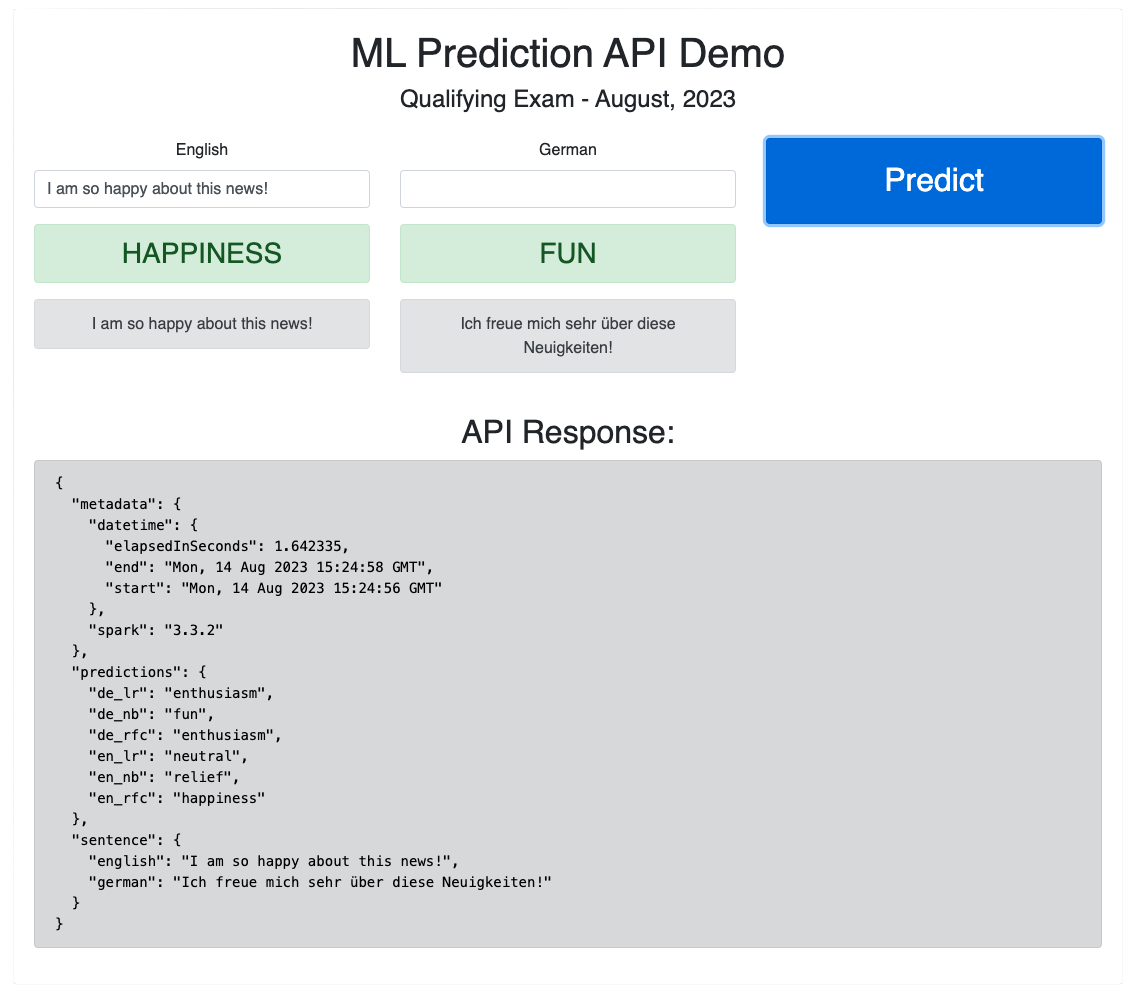
\includegraphics[width=0.85\textwidth]{images/Demo-Api-2.png}
    \caption{Demo API Webpage}
    \label{fig:demo-api-webpage}
\end{figure}

In the screenshot (Figure: \ref{fig:demo-api-webpage}) example a sentence was entered in the English text-box and the "Predict" button pressed. The API took about $\sim$1.6seconds to translate the English to German and then process both sentences on the pre-trained ML models, build the \texttt{JSON} object and return it to the application.

\subsection{Written \& Oral Presentation of Research Finding}
In conclusion of the project a research paper and oral presentation is required to pass the  MTSU Computation Data Science PhD Qualifying Exam. The listing of all the datasets used, code for the application, and details of the research project process in this research paper is openly available and hosted on a GitHub repository, allowing for easy access, reproducible, and collaborative engagement with the research findings. The repository is open and available under: \texttt{https://github.com/richardhoehn/mtsu.coms.qualifying-exam}\cite{Hoehn_Improving_Emotion_Detection_2023}. In addition of all the code being listed in a public repository the paper was comprised and build using \LaTeX\footnote{LaTeX UR: https://www.latex-project.org/}.

Using \LaTeX\;for this paper provides numerous benefits, some of which are portability, source control (due to plain-text nature), bibliography management, and last but not least the ability to write clean mathematical equations. 

\clearpage
\section{Results and Analysis}
\label{sec:results-and-analysis}
This section lists the prediction rates of training and testing of the original and extended datasets both in English and German. Overall results seem to indicate that there was no measurable benefit and even negative outcomes from adding the extended data for Emotion Detection. In the subsections details on the results are listed by the common standards of using the below equations \ref{eq:accuracy}, \ref{eq:precision}, \ref{eq:recall}, and \ref{eq:f1-score} for Accuracy, Precision, Recall, and the F1 Score. It should be noted that ED is a multi-class classification problem, which means that the machine learning process assigns the predictions from the sentence data to one of several predefined emotion categories (see Table \ref{table:dataset_labels}).

\subsection{Prediction Results of Original \& Extended Datasets}
Overall the prediction results from the trained models is disappointing. Using the Random Forrest Classifier described in Section \ref{sec:evaluation-metrics-and-methodologies} provided the best prediction results based on a combination of the Accuracy and the F1 Score. It should be noted although the accuracy may be slightly better on the GLM models for both English and German, if one reviews the F1 Score, the RFC model performs better.

Oddly, the prediction results with the extended data where lower than using the original (non-extended) data for training. In the Analysis and Conclusions section \ref{sec:analysis-of-impact-of-extending-datasets} details on why this may be the case are discussed in detail.

\subsubsection{Formulas and Equations used in Analysis}
The accuracy (eq: \ref{eq:accuracy}) of any machine learning model is a clear and easily comprehend-able way to understand the performance of a model. However, it is important to consider the context and potential trade-offs with other metrics, as high accuracy alone might not adequately capture the full picture of a model's performance. This can be especially true for multi-class classification models such as the ED analysis that we are working on.

\begin{equation}
Accuracy = \frac{TP+TN}{TP+TN+FP+FN}
\label{eq:accuracy}
\end{equation}

The Precision (eq: \ref{eq:precision}) focuses in detail on the accuracy of positive predictions (TP)\footnote{Positive Predictions = TP (True Positive)} made by the model. According to Google Cloud's definition, precision answers the question: What proportion of positive predictions were actually correct?

\begin{equation}
Precision = \frac{TP}{TP+FP}
\label{eq:precision}
\end{equation}

Since our project is a multi-class classification project we will need to utilize Micro Averaging for the Precision. With this in mind, we extend our simple equation \ref{eq:precision} for precision to incorporate micro averaging as defined in equation 
\ref{eq:precision_micro_avg}.

\begin{equation}
Precision_{MicroAvg} = \frac{(TP_1 + TP_2 + \ldots + TP_n)}{(TP_1 + TP_2 + \ldots + TP_n + FP_1 + FP_2 + \ldots + FP_n)}
\label{eq:precision_micro_avg}
\end{equation}

The Recall (eq: \ref{eq:recall}) focuses on the in detail on the accuracy of positive predictions\footnote{Negative Predictions = FN (False Negative)} made by the model. Per Google Cloud's definition: The recall attempts to answer: What proportion of actual positives.

\begin{equation}
Recall = \frac{TP}{TP+FN}
\label{eq:recall}
\end{equation}

Since our project is a multi-class classification project we will need to actually use Micro Averaging for the Recall in a similar fashion to how we used it on Precision. With this in mind we extend our simple equation \ref{eq:recall} of recall to incorporate micro averaging as defined in equation \ref{eq:recall_micro_avg}.

\begin{equation}
Recall_{MicroAvg} = \frac{(TP_1 + TP_2 + \ldots + TP_n)}{(TP_1 + TP_2 + \ldots + TP_n + FP_1 + FP_2 + \ldots + FP_n)}
\label{eq:recall_micro_avg}
\end{equation}

The F1 Score (eq: \ref{eq:f1-score}) in our project is important to assess the balance between precision and recall. In addition, the F1 Score holds significance in multi-class classification scenarios where there are more than two classes.

\begin{equation}
F1_{Score} = \frac{2*Precision*Recall}{Precision+Recall}
\label{eq:f1-score}
\end{equation}

Lastly, we employed micro averaging for the Recall, Precision, and F1 Score due to the fact that it assigns equal weight to each label (Emotion, as seen in Table \ref{table:dataset_labels}), regardless of the class label and the number of labels taken into account. This approach ensures that the evaluation metrics give uniform importance to all labels, making it particularly suitable for scenarios where class imbalances exist or where an fair assessment of model performance across all emotion classes is required.

\subsubsection{English Dataset Results}
\label{sec:english-dataset-results}
The Table \ref{table:en_testing_results} lists the results of all three ML models, their accuracy and F1 Score based on the English original and extended datasets. The improvements from the original and extended datasets are listed in the last column. In all cases the improvement to using the extended datasets was negative.

\begin{table}[h!]
\centering
\begin{tabular}{ | L | M | M | M | M | M | }
    \hline
    \multicolumn{6}{|c|}{Results of English Dataset} \\
    \hline
    &
    \multicolumn{2}{c|}{Original Dataset} &
    \multicolumn{3}{c|}{Extended Dataset} \\
    & Accuracy & F1 Score & Accuracy & F1 Score & Improvement \\
    \hline
    Random Forrest & 
    29.72\% &
    25.83\% & 
    21.23\%  &
    19.43\% &
    -28.56\% \\
    \hline
    Na\"ive Bayes & 
    5.66\% &
    6.92\% & 
    3.77\%  &
    4.14\% &
    -33.39\% \\
    \hline
    GLM (lr) & 
    32.08\% &
    23.68\% & 
    25.47\%  &
    16.19\% &
    -19.95\% \\
    \hline
\end{tabular}
\caption{Model Testing Results on English Dataset}
\label{table:en_testing_results}
\end{table}

\subsubsection{German Dataset Results}
\label{sec:german-dataset-results}
The Table \ref{table:de_testing_results} lists the results of all three ML models, their accuracy and F1 Score based on the German original and translated from English to German extended datasets. The improvements from the original and extended datasets are listed in the last column. Interestingly the Random Forrest Classifier was the only negative improvement whereas the GLM and Naive Bayes models had improvements. However it should be noted that the prediction rates are so low in the GLM and Naive Bayes that they should not really be considered improvements.

\begin{table}[h!]
\centering
\begin{tabular}{ | L | M | M | M | M | M | }
    \hline
    \multicolumn{6}{|c|}{Results of German Dataset} \\
    \hline
    &
    \multicolumn{2}{c|}{Original Dataset} &
    \multicolumn{3}{c|}{Extended Dataset} \\
    & Accuracy & F1 Score & Accuracy & F1 Score & Improvement \\
    \hline
    Random Forrest & 
    28.10\% &
    16.84\% & 
    25.71\%  &
    18.56\% &
    -8.50\% \\
    \hline
    Na\"ive Bayes & 
    4.29\% &
    4.31\% & 
    6.67\%  &
    4.21\% &
    +55.48\% \\
    \hline
    GLM (lr) & 
    34.29\% &
    17.57\% & 
    24.76\%  &
    18.27\% &
    -27.79\% \\
    \hline
\end{tabular}
\caption{Model Testing Results on German Dataset}
\label{table:de_testing_results}
\end{table}

The improvements on the accuracy are based on Equation \eqref{eq:improvement} listed below. It is a simple and straightforward way of comparing the Accuracy from the original trained dataset to the extended trained dataset for purposes of comparing the potential benefits of extending the training datasets by translation.

\begin{equation}
Improvement(\%) = \dfrac{(Accuracy_{Ext} (\%) - Accuracy_{Org} (\%))}{Accuracy_{Org}(\%)}
\label{eq:improvement}
\end{equation}

It should be noted that although the improvement values are fairly large negatives those come from the fact that the accuracy is small and in most all cases the accuracy is around the 25 - 30\% values and a change of just a few percent can have a significant impact on the improvement values.

\subsection{Analysis of the impact of Extending Datasets by Translation}
\label{sec:analysis-of-impact-of-extending-datasets}
While extending datasets for machine learning training can often improve\cite{Sarker2021} model performance, it's important to recognize that this approach has its limitations, especially in ML models that can reach a limit on training data. In our case, relying on translation services for dataset expansion might not consistently yield better results when extending the data from translated text. These services, in our case using Google Translate\footnote{Google Cloud Translate URL: https://cloud.google.com/translate} can introduce errors or inaccuracies in translations especially in the context of emotions of a particular text, leading to noisy or incorrect training data. Consequently, the models may learn from erroneous information, which did negatively impact our models performance on the ED tasks.

Specifically in our case of extending the original English and German datasets with translated data seems to indicate that the sentences and structure are not the same and therefore the prediction rates went down as the models got more diluted.


\subsection{Impact Using API for Real-Time Translation}
\label{sec:impact-using-api-for-real-time-translation}
With the help of the webpage (Figure \ref{fig:demo-api-webpage} on \pageref{fig:demo-api-webpage}) a sense of the inaccuracy was also presented. Each round trip to the API took an between 1.4 and 1.6seconds. The prediction results mirrored those of Tables \ref{table:en_testing_results} and \ref{table:de_testing_results} which in turn made the usefulness of the translation not practical as can be seen in Table \ref{table:api-test-results} below.


\begin{table}[h!]
\centering
\begin{tabular}{ | N | M | L | N | L | N | }
    \hline
    \multicolumn{6}{|c|}{Webpage API Test} \\
    \hline
     & 
    \multicolumn{2}{c|}{English} &
    \multicolumn{2}{c|}{German} & 
     \\
    \hline
    Test &
    Emotion & Sentence &
    Emotion & Sentence &
    Time \\
    \hline
    A &
    Worry & This is bad idea and we need to stop right now &
    Anger & Dies ist eine schlechte Idee und wir müssen jetzt aufhören &
    1.49s \\
    \hline
    B &
    Happiness & What a wonderful world this is! &
    Relief & Was fur eine wundervolle Welt das ist! &
    1.65s \\
    \hline
    C &
    Happiness & I am so happy about this news! &
    Fun & Ich freue mich sehr uber diese Nauigkeiten! &
    1.64s \\
    \hline
    D &
    Sadness & Gosh I hate doing this today. &
    Relief & Meine Güte, ich hasse es heute. &
    2.56s \\
    \hline
\end{tabular}
\caption{API Webpage Test Results}
\label{table:api-test-results}
\end{table}

\subsection{Findings and Implications for Improving Emotion Detection}
\label{sec:findings-and-implications-for-improving}
Based on the improvement results in Sections \ref{sec:english-dataset-results} and \ref{sec:german-dataset-results} it seems that using translation to extend both the English and German datasets resulted in a negative outcomes. The best outcomes were using a simple Linear Regression model on the English and German, however based on the F1 Score (Eq: \ref{eq:f1-score}) of the Random Forest Classifier it seems to perform the best on both English and German. This is because the false positive amount of one score on the accuracy is not taken into account and can easily skew the results when using a multi-class classification model.

Considering the outcomes of data extension via translation, our approach of utilizing real-time translation for multi-language models through the creation of an API and translating text in real-time for both German and English appears to be unsatisfactory in terms of achieving any substantial improvement as well.

With both these findings, we believe that the data of only using $\sim$1,500 (original dataset) and $\sim$2,700 (extended dataset) to train models is insufficient\cite{overfitting-overview} when using a multi-class classification problem. By inference, if we have only 1,500 and divide (eq: \ref{eq:sentence-per-class}) those by our eight (Table: \ref{table:dataset_labels}) classes we simply do not have enough data to truly train the ML on the classes.

\begin{equation}
\begin{split}
\frac{Features}{Labels}= \frac{Sentences}{Classes}=\frac{1,500}{8}=185 \\
or=\frac{2,700}{8}=337
\end{split}
\label{eq:sentence-per-class}
\end{equation}

Taking into account the insufficiency of data, the implication of a lack of classified data can lead to several significant issues for our ML models. Firstly, there's an absence of context for the models to operate effectively and grasp the intricate nuances of both the English and German languages. Secondly, in cases where class data is lacking, the models tend to memorize existing sentences and words, rather than learning the underlying patterns of the language. Both of these issues are connected to a phenomenon called overfitting\cite{overfitting-overview}, which is prevalent in many regression problems.

Options for improvement range from the straightforward approach of acquiring more data to the more nuanced strategy of leveraging existing labeled sentences and employing machines to generate derivatives. This would facilitate the creation of more intricate patterns for the machines to learn from. 

\subsection{Conclusion and Future Work}
It's crucial to ensure the quality and accuracy of extended data, especially when language translation is involved, to prevent introducing more noise than meaningful information into the training process. The implications of the lack of data in ED analysis presented itself in this research that sought to try and overcome these issues. Although the research did not yield any significant improvements through translating the German to English as a means of extending the English dataset, it ultimately worsened the prediction results. We believe one of the main culprits is that the data for learning based on eight classes was insufficient. As can be seen in Equation \ref{eq:sentence-per-class} from Section \ref{sec:findings-and-implications-for-improving}, the models seemingly resorted to memorizing the sentence rather than learning the intricacies of the labeled classes. This inference arises that certain labels exhibited better F1 Score performance, primarily due to their greater availability in the training data.

Two areas of prospective research emerge: firstly, conducting further tests involving the translation of different models using diverse translation services. While Google Cloud's translation service sufficed for this research, superior paid subscription-based translation services are available. With the help of more data and better translation more concrete answers to improving predictions may be achieved. Secondly, another avenue to overcome the lack of data involves employing AI to generate sentences that are similar yet distinct from the original. This could be achieved by providing a sentence and its associated labeled class to the AI for data creation. This approach aims to produce additional sentences imbued with similar emotional attributes, potentially expanding the labeled dataset.

\clearpage
\addcontentsline{toc}{section}{References}
\printbibliography
\clearpage


\addcontentsline{toc}{section}{List of Figures}
\listoffigures
\clearpage


% Appendix Details
\appendix
\section{Appendix -- Dataset Details}
The following details in this appendix are for clarification purposes.
All examples in this appendix are created via PySpark using dataframes.

\subsection{Using PySpark to Load Data}
All example code was created using Jupyter Notebooks creating a PySpark session. The details of setting up such session are below in the code example. All subsequent details are derived from the \texttt{sc}\footnote{sc = Spark Session}.
\begin{minted}[fontsize=\small]{python}
# General Imports
import glob
import shutil

# Setup Spark Session
from pyspark.sql import SparkSession

# Get Spark Functions Needed
from pyspark.sql.functions import col, udf, split, explode

# Get Datatypes needed for DataFrame manipulation
from pyspark.sql.types import IntegerType, StringType

# Setup Spark Session
sc = SparkSession \
        .builder \
        .master("local[*]") \
        .appName("data_clean_up") \
        .getOrCreate()

# Print Spark Version being run
print("Spark V: ", sc.version)
\end{minted}
\clearpage


\subsection{Details on English Dataset}
\label{appendix:dataset_english}
The English dataset is based on tweets\footnote{Tweets from Twitter} that are saved as a \texttt{csv}\footnote{csv = Comma Separated Values} file. The following code was use to filter and process the file for use in this project.
\begin{minted}[fontsize=\small]{python}
# *********************************
# *** English Data Preparations ***
# *********************************

# Load English CSV File into a Dataframe
df_english = sc.read.csv("data/english.csv", header=True, inferSchema=True)
print(f'Count (raw): {df_english.count()}')

# Print Columns
print(f'English Source Columns: {df_english.columns}\n')

# Filter only lavbels that we mathc with the German counter parts
filter_values = ["love", "hate", "neutral", "anger", "happiness", "surprise", "sadness", "worry", "enthusiasm"]
df_english_filtered = df_english.filter(col("sentiment").isin(filter_values))

# Remove unnecessary column
df_english_filtered = df_english_filtered.drop("tweet_id")

# Rename Columns
df_english_filtered = df_english_filtered.withColumnRenamed("sentiment", "emotion_en")
df_english_filtered = df_english_filtered.withColumnRenamed("content", "sentence_en")

# Make sure the column order to the same for both german and english csv files
df_english_filtered = df_english_filtered.select('sentence_en', 'emotion_en')

print(f'Count (filtered): {df_english_filtered.count()}')

# Group By for Details & Count
df_english_grouped = df_english_filtered.groupBy('emotion_en').count()

# Show Groupings and Respetive Counts
print('\nGrouped & Count by "emotion"')
df_english_grouped.show(truncate=0)


# Save Dataframe to CSV
directory_path = 'data/spark_data_parts'
df_english_filtered.coalesce(1).write.csv(directory_path, header=True, mode="overwrite")

file_pattern = 'part-00000*.csv'
file_path = glob.glob(directory_path + '/' + file_pattern)[0]

shutil.move(file_path, './data/data_en.csv')

Count (raw): 40000
English Source Columns: ['tweet_id', 'sentiment', 'content']

Count (filtered): 35692

Grouped & Count by "emotion"
+----------+-----+
|emotion_en|count|
+----------+-----+
|love      |3842 |
|hate      |1323 |
|neutral   |8638 |
|anger     |110  |
|happiness |5209 |
|surprise  |2187 |
|sadness   |5165 |
|worry     |8459 |
|enthusiasm|759  |
+----------+-----+
\end{minted}
\clearpage

\subsection{Details on German Dataset}
\label{appendix:dataset_german}
The German dataset was downloaded from the ETH's\footnote{ETH (German: Eidgenössische Technische Hochschule) or Swiss Federal Institute of Technology} servers via "link" as a \texttt{JSON} file. Since the the file was \texttt{JSON} we will need to filter and explode the file based on teh emotions that are attached to it.
\begin{minted}[fontsize=\small]{python}
# ********************************
# *** German Data Preparations ***
# ********************************

# Load German JSON File into a Dataframe
df_german = sc.read.json("data/german.json")
print(f'Count (raw): {df_german.count()}')

# Print Columns
print(f'German Source Columns: {df_german.columns}\n')


# We Need to "split" the "artice_emotion" column since the ETH team listed
# multiple emotions in one column
# In order to "explode" the column to it's distinct rows
df_german_exploded = df_german.select('*', explode('article_emotion').alias('emotion_de'))

# Rename Column
df_german_exploded = df_german_exploded.withColumnRenamed("title", "sentence_de")

# Remove unnecessary column
df_german_exploded = df_german_exploded.drop("article_id")
df_german_exploded = df_german_exploded.drop("article_stance")
df_german_exploded = df_german_exploded.drop("paragraphs")
df_german_exploded = df_german_exploded.drop("source")
df_german_exploded = df_german_exploded.drop("article_emotion")
df_german_exploded = df_german_exploded.drop("snippet")

# Make sure the column order to the same for both german and english csv files
df_german_exploded = df_german_exploded.select('sentence_de', 'emotion_de')

print(f'Count (filtered): {df_german_exploded.count()}')

# Group By for Details & Count
df_german_grouped = df_german_exploded.groupBy('emotion_de').count()

# Show Groupings and Respetive Counts
print('\nGrouped & Count by "emotion"')
df_german_grouped.show(truncate=0)


# Save Dataframe to CSV
directory_path = 'data/spark_data_parts'
df_german_exploded.coalesce(1).write.csv(directory_path, header=True, mode="overwrite")

file_pattern = 'part-00000*.csv'
file_path = glob.glob(directory_path + '/' + file_pattern)[0]

shutil.move(file_path, './data/data_de.csv')

Count (raw): 1970
German Source Columns: ['article_emotion', 'article_id', 'article_stance', 'paragraphs', 'snippet', 'source', 'title']

Count (filtered): 2568

Grouped & Count by "emotion"
+------------+-----+
|emotion_de  |count|
+------------+-----+
|Vertrauen   |316  |
|Freude      |140  |
|Ärger       |226  |
|Überraschung|369  |
|Traurigkeit |184  |
|Antizipation|774  |
|Unklar      |314  |
|Angst       |154  |
|Ekel        |29   |
|Keine       |62   |
+------------+-----+
\end{minted}
\clearpage


\subsection{Details on Extending \& Translation}
\label{appendix:dataset_translation}
Details on translation and extending the datasets.
\begin{minted}[fontsize=\small]{python}
# **************************************
# *** English <-> German Emotion Key ***
# **************************************


from pyspark.sql.functions import col, udf, split, explode, lit
from pyspark.sql.types import IntegerType, StringType, StructType, StructField, StringType

# Emotion Dictionary English <-> German
# This key/value setup was previsoulsy created for linking purposes
emotion_key = {
    "boredom"    : "---",
    "love"       : "Vertrauen",
    "relief"     : "---",
    "fun"        : "---",
    "hate"       : "Ekel",
    "neutral"    : "Unklar",
    "anger"      : "Ärger",
    "happiness"  : "Freude",
    "surprise"   : "Überraschung", 
    "sadness"    : "Traurigkeit", 
    "worry"      : "Angst",
    "enthusiasm" : "Antizipation", 
    "empty "     : "---",
    "---"        : "Keine",
}

# Create the schema for the DataFrame
schema = StructType([
    StructField("emotion_en", StringType(), nullable=False),
    StructField("emotion_de", StringType(), nullable=False)
])

# Convert the dictionary to a list of tuples
data = [(key, value) for key, value in emotion_key.items()]

# Create the PySaprk DataFrame
df_emotion_key = sc.createDataFrame(data, schema)

df_emotion_key.show()

# Extend the English and German onto the datasets
df_german_exploded = df_german_exploded.join(df_emotion_key, on="emotion_de", how="left")
df_english_filtered = df_english_filtered.join(df_emotion_key, on="emotion_en", how="left")

# New sentence column
df_german_exploded = df_german_exploded.withColumn("sentence_en", lit(None))
df_english_filtered = df_english_filtered.withColumn("sentence_de", lit(None))

df_german_exploded.show()
df_english_filtered.show()


# Using Deep Translator to proxy to Google Translate
from deep_translator import GoogleTranslator


# Define Tranlation Functions
def translate_en_to_de(row):
    translated = GoogleTranslator(source='en', target='de').translate(row["sentence_en"])
    row["sentence_de"] = translated

def translate_de_to_en(row):
    translated = GoogleTranslator(source='de', target='en').translate(row["sentence_en"])
    row["sentence_en"] = translated
    

df_german_exploded.foreach(translate_de_to_en)  

+----------+------------+
|emotion_en|  emotion_de|
+----------+------------+
|   boredom|         ---|
|      love|   Vertrauen|
|    relief|         ---|
|       fun|         ---|
|      hate|        Ekel|
|   neutral|      Unklar|
|     anger|       Ärger|
| happiness|      Freude|
|  surprise|Überraschung|
|   sadness| Traurigkeit|
|     worry|       Angst|
|enthusiasm|Antizipation|
|    empty |         ---|
|       ---|       Keine|
+----------+------------+

+------------+--------------------+----------+----------+-----------+----------+
|  emotion_de|         sentence_de|emotion_en|emotion_en|sentence_en|emotion_en|
+------------+--------------------+----------+----------+-----------+----------+
|   Vertrauen|Adoptiert zu sein...|      love|      love|       null|      love|
|      Freude|Österreichs Verfa...| happiness| happiness|       null| happiness|
|      Freude|Visana gewinnt er...| happiness| happiness|       null| happiness|
\end{minted}
\clearpage
 % Note: SubSection headers are handled within the *.tex file 
\section{Appendix -- Application \& Code Details}
Hello World - Application \& Code Details
\subsection{Application}
\label{appendix:code_application}
Hello World - Application
\clearpage

\subsection{Code Details}
Hello World - Code Details

\subsection{RESTful API Server}
\label{appendix:code-api-server}
The RESTful\footnote{RESTful API is an interface that two computer systems use to exchange information securely over the internet.} API Server will be a simple Python Flask server listening on port \texttt{8080} on the local machine.


\clearpage
 % Note: SubSection headers are handled within the *.tex file 

\end{document}



